% Prof. Dr. Ausberto S. Castro Vera
% UENF - CCT - LCMAT - Curso de Ci\^{e}ncia da Computa\c{c}\~{a}o
% Campos, RJ,  2022
% Disciplina: An\'{a}lise e Projeto de Sistemas
% Aluno:


\chapterimage{planejamento.png} % Table of contents heading image
\chapter{Etapa de Planejamento}


Este capítulo apresenta o requisito do sistema, seus benefícios e um estudo de viabilidade de desenvolvimento do projeto para definir se o sistema possível.


\section{Solicita\c{c}\~{a}o do Sistema}
%%%%%%%%%%%%%%%%%%%%%%%%%%%%%%%


\begin{itemize}

      \item \textit{Responsável}

            – Daniel Terra Gomes

      \item \textit{Necessidade da Empresa }

            - Este projeto visa viabilizar, facilitar e agilizar os processos e atividades da rede de um Empresa que trabalha com veículos autônomos de forma a promover uma melhor localização dos veículos, eficiência no trabalho dos colaboradores, e eficiência de transportes.

      \item \textit{Requisitos
                  de negócios}


            - O sistema será capaz de cadastrar, classificar e controlar os veículos que estão à disposição do sistema. Capture, filtre e extraia dados relevantes de informações relacionados ao carros da empresa e da demanda de uso desses veículos. Dessa forma podendo analisar esses dados e fazer alterações a partir da demanda.

            - O sistema permitirá que os clientes solicitem os veículos através do nosso App de celular, após a solicitação do veículo será feita a confirmação dos dados do usuário, validação das informações de pagamento. Assim, com os dados conferidos o envido do carro autônomo será alocado no sistema. Dessa forma, o veículo mais próximo disponível do usuário será enviado para a viagem.

            - Também serão levados em conta o gasto com a organização, montagem dos equipamentos e recursos necessários à utilização do sistema.

            - Controlar, pesquisar e gerenciar bancos de dados contendo: informações dos veículos, tempo de uso, manutenção, funcionários, viagens, clientes e locações.

            - Fornecimento de meios de comunicação, relacionamento com clientes por meio de atendimento online, locação online via App.


      \item \textit{Valor
                  agregado}

            - Com as locações dos veículos e suas disponibilidades estão sob controle do banco de dados, espera-se que as despesas com gerenciamento de recursos sejam reduzidas, permitindo um melhor acompanhamento e controle dos veículos da empresa. Ao analisar os dados dos usuários cadastrados no sistema podemos gerar modelos preditivos assim oferecendo promoções para certas localizações que a empresa atua. Dessa forma, espera-se uma ampliação e fidelização da base de clientes, o que resultará em um consequente aumento no lucro da empresa.

      \item \textit{Outra
                  informações}

            - Por se tratar de um sistema rico em funcionalidades e complexo, uma parte importante do trabalho será a estruturação o sistema de comunicação remoto com as interface do aplicativo que faz a  comunicação com usuário e os veículos da empresa, de forma a facilitar a transição de processos manuais para o uso do sistema e conseguir agilizar efetivamente todos os processos realizados pela rede, além de agilizar o relacionamento e a troca de dados entre eles.

\end{itemize}

\section{Custos: Desenvolvimento e Operacional}
%%%%%%%%%%%%%%%%%%%%%%%%%%%%%%%
\begin{itemize}
      \item \textit{Desenvolvimento}

            - Salário da equipe de desenvolvimento;

            - Custos de licenças de hardware e software a serem usadas;

            - Treinamento e qualificação da equipe de desenvolvimento e dos funcionários;

            - Despesas de escritório;

            - Equipamentos para escritório.



      \item \textit{Operacional}

            - Salário da equipe operacional;

            - Custos de instalação do sistema;

            - Gastos com energia elétrica;

            - Treinamento de funcionários;

            - Reparo e atualização de hardware;

            - Licenciamento de Software;

            - Atualização de software e serviços de comunicação.

\end{itemize}
\section{Benef\'{\i}cios}
%%%%%%%%%%%%%%%%%%%%%%%%%%%%%%%
Nesta seção, os benefícios tangíveis e intangíveis que o sistema proporcionará são identificados e detalhados a seguir:

\subsection{Benef\'{\i}cios Tang\'{\i}veis}
\begin{itemize}

      \item \textit{Sistema mais rápido}
      \item \textit{Aumento nas solicitações dos veículos}
      \item \textit{Otimização dos processos empresariais}
      \item \textit{Facilitação da da localização dos veículos}
      \item \textit{Aumento na eficácia dos processos}
      \item \textit{Aumento das viagens}
      \item \textit{Aumento do lucro geral da empresa}



\end{itemize}

\subsection{Benef\'{\i}cios Intang\'{\i}veis}
\begin{itemize}

      \item \textit{Maior abrangência de mercado}
      \item \textit{Aumento do reconhecimento da marca}
      \item \textit{Conquista de novo público}
      \item \textit{Melhora do serviço ao cliente}
      \item \textit{Aumento do bem estar no ambiente de trabalho e em nossos veículos}
      \item \textit{Clientes mais satisfeitos}



\end{itemize}






\section{Estudo de Viabilidade}
%%%%%%%%%%%%%%%%%%%%%%%%%%%%%%%
Esta seção examina os aspectos que afetam a viabilidade do projeto e leva a uma conclusão. Ademais, o cronograma das atividades que serão realizadas para a construção do sistema e a execução do cálculo do custo total do projeto são apresentados a seguir. Essas informações podem ser usadas para determinar a viabilidade do projeto.

\subsection{Calend\'{a}rio }

\begin{table}[H]
      \begin{center}
            \caption{Calendário com as fases de construção do sistema} \label{tabela1}
            \begin{tabular}{lrc}
                  \hline
                  FASE              & DATA                    \\
                  \hline
                  Início do projeto & 01 de Agosto de 2022    \\
                  Planejamento      & 25/08/2022 á 22/09/2022 \\
                  Análise           & 23/09/2022 á 23/12/2022 \\
                  Projeto           & 14/01/2023 á 14/02/2023 \\
                  Implementação     & 24/02/2023 á 24/07/2023 \\
                  Conclusão         & 01 de Agosto de 2023    \\
                  \hline
            \end{tabular}
      \end{center}
\end{table}

\subsection{Cronograma }
\begin{figure}[H]
      \begin{center}
            \caption{Cronograma do Projeto } \label{afp}

            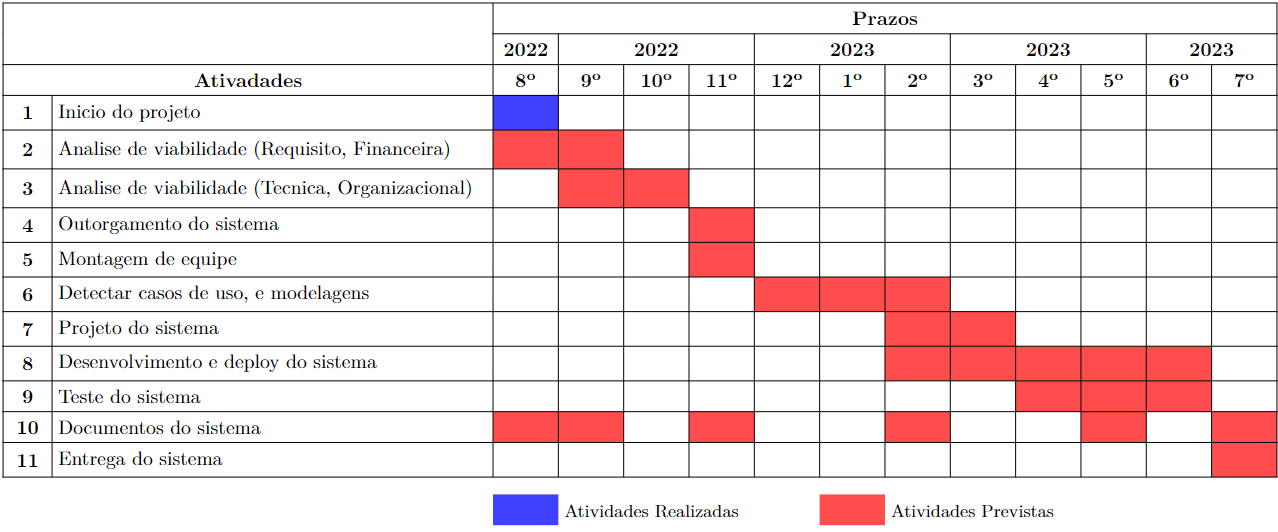
\includegraphics[width=15cm]{Cronograma.png} \\
      \end{center}
\end{figure}



\subsection{Or\c{c}amento } \label{orcamento}
Segue abaixo a tabela referente ao orçamento do sistema. Nele encontramos o número de componentes, o nome desses componentes, o preço unitário e o número de componentes necessários, bem como o valor total do orçamento.

\begin{tabular}{ |p{3cm}||p{3cm}|p{3cm}|p{3cm}|  }
      \hline
      \multicolumn{4}{|c|}{Or\c{c}amento}                                                                                                                                                 \\
      \hline
      \textbf{Quantidade} & \textbf{Componentes}                                                                          & \textbf{Preço/unidade} & \textbf{Valores \$}                  \\
      \hline
                          & \textbf{Hardware}                                                                             &                        &                                      \\
      1                   & Terceirizada (componentes na Seção \ref{Hardware})                                            & -                      & 1,000,000                            \\
      27                  & Starlink Satélites de comunicação (Plano Anual Business para todos os 27 estados brasileiros) & 12,000,000             & 324,000,000                          \\
      2700                & Torres 5G de comunicação                                                                      & 50,000                 & 135,000,000                           \\
      3000                & Carros                                                                                        & 130,000                & 390,000,000                          \\
                          & \textbf{Software}                                                                             &                        &                                      \\
      3                   & Sistemas operacionais proprietário                                                            & -                      & 100,000                              \\
                          & \textbf{Pessoas}                                                                              &                        &                                      \\
      20                  & Programadores                                                                                 & 4,000,000              & 80,000                               \\
      4                   & Analista de sistema                                                                           & 8,00,000               & 32,000                               \\
      2                   & Chefe do Projeto                                                                              & 30,000,000             & 60,000                               \\
      4                   & Arquitetos de software                                                                        & 11,000,000             & 44,000                               \\
      2                   & Projetista                                                                                    & 4,000,000              & 8,000                                \\
      1                   & Avaliadores de Qualidade                                                                      & 2,000,000              & 2,000                                \\
      5                   & Funcionários de manutenção                                                                    & 3,000,000              & 15,000                               \\
      4                   & Engenheiro de Inteligencia Artificial                                                         & 14,000,000             & 56,000                               \\
      2                   & Cientista de Inteligencia Artificial                                                          & 10,000,000             & 20,000                               \\
      \hline
                          &                                                                                               &                        & \textbf{Valor total \$:} 728,919,000
      \\
      \hline
\end{tabular}

\subsection{Resumo e Recomenda\c{c}\~{o}es}
É de suma importância que seja seguido o cronograma proposto na tabela \ref{orcamento}, dessa mesma forma todos os equipamentos necessários devem ser adquiridos. Essas recomendações são extremamente necessárias para a elaboração correta do sistema proposto.
Recomenda-se ainda levar em consideração que o cronograma de tarefas do sistema em desenvolvimento atende aos requisitos, e os custos de construção cabem no orçamento do empreendimento, bem como a manutenção dos equipamentos levantados durante o projeto para a criação de o sistema. Isso torna o projeto viável técnica, econômica e organizacionalmente.
